Niniejszy podrozdział przedstawia różne badania, których celem jest ewaluacja klasyfikacji YOLOv8n na przykładzie klasy człowiek. Model zbadano pod kątem wpływu jak manipulacja poziomem oświetlenia oraz progu ufności przekłada się na jego wyniki. Dla każdego zmierzonego progu ufności wyznaczane będą metryki potrzebne do zobrazowania wniosków. Będą one liczone na podstawie poprzednio uzyskanych metryk --- TP, TN, FP i FN. Do testu wykrzystano cztery filmy. Każdy z nich przedstawia wyłącznie człowieka. Wartości jasności i nasycenia przedstawiono w tabeli \ref{tab:saturacja-jasnosc-czlowiek}. Wygląd nagranego pomieszczenia dla różnych poziomów oświetlenia ukazano na rysunku \ref{fig:person_grid}. 
\begin{table}[H]
\centering
\caption{Jasność i nasycenie dla wszystkich filmów.}
\begin{tabular}{|c|c|c|c|}
\hline
Poziom oświetlenia  & Obecne obiekty & Jasność & Nasycenie \\ \hline
1        & człowiek       & 152.73  & 107.3     \\ \hline
2        & człowiek       & 134.64  & 93.48     \\ \hline
3        & człowiek       & 41.59   & 123.48    \\ \hline
4        & człowiek       & 25.47   & 90.92     \\ \hline
\end{tabular}

\label{tab:saturacja-jasnosc-czlowiek}
\end{table}








\subsection{Ewaluacja modelu dla różnych poziomów oświetlenia}
\label{sec:test-AUC}
W sekcji tej oceniono osiągi modelu dla każdego poziomu oświetlania, a następnie porównano jest ze sobą. Do wizualizacji wyników posłużono się krzywą ROC, zaś do oceny rezultatów dla poziomu jasności -- wartością AUC.

Krzywa ROC (ang. \emph{Receiver operating characteristic}) to graficzna reprezentacja wykorzystywana do ewaluacji binarnej klasyfikacji modelu. Jest to zbiór połączonych ze sobą punktów o współrzędnych $(x, y)$. Liczba narysowanych punktów odpowiada liczbie przetestowanych progów ufności. Współrzędna $x$ to metryka FPR, a współrzędna $y$ -- TPR. Przykład wyznaczonych punktów pokazuje tabela \ref{tab:wyznaczanie_ROC}. 
    \begin{table}[H]
        \centering
    \caption{Przykład wyznaczania punktów krzywej ROC}

        \begin{tabular}{|c|c|c|c|c|c|c|c|}
        \hline
        Próg   ufności & TP & TN & FP & FN & FPR  & TPR  & Punkt na   wykresie \\ \hline
        0              & 60 & 0  & 26 & 0  & 1    & 1    & (1, 1)              \\ \hline
        0.01           & 55 & 0  & 26 & 5  & 1    & 0.92 & (1, 0.92)           \\ \hline
        0.02           & 38 & 3  & 23 & 22 & 0.88 & 0.63 & (0.88, 0.63)        \\ \hline
        0.03           & 22 & 13 & 13 & 38 & 0.5  & 0.37 & (0.5, 0.37)         \\ \hline
        0.04           & 18 & 16 & 10 & 42 & 0.38 & 0.3  & (0.38, 0.3)         \\ \hline
        0.05           & 11 & 19 & 7  & 49 & 0.27 & 0.18 & (0.27, 0.18)        \\ \hline
        0.06           & 8  & 21 & 5  & 52 & 0.19 & 0.13 & (0.19, 0.13)        \\ \hline
        0.07           & 6  & 22 & 4  & 54 & 0.15 & 0.1  & (0.15, 0.1)         \\ \hline
        0.08           & 5  & 22 & 4  & 55 & 0.15 & 0.08 & (0.15, 0.08)        \\ \hline
        0.09           & 3  & 23 & 3  & 57 & 0.12 & 0.05 & (0.12, 0.05)        \\ \hline
        0.1            & 3  & 23 & 3  & 57 & 0.12 & 0.05 & (0.12, 0.05)        \\ \hline
        0.11           & 3  & 24 & 2  & 57 & 0.08 & 0.05 & (0.08, 0.05)        \\ \hline
        0.12           & 3  & 25 & 1  & 57 & 0.04 & 0.05 & (0.04, 0.05)        \\ \hline
        0.13           & 3  & 25 & 1  & 57 & 0.04 & 0.05 & (0.04, 0.05)        \\ \hline
        0.14           & 3  & 25 & 1  & 57 & 0.04 & 0.05 & (0.04, 0.05)        \\ \hline
        0.15           & 3  & 25 & 1  & 57 & 0.04 & 0.05 & (0.04, 0.05)        \\ \hline
        0.16           & 3  & 25 & 1  & 57 & 0.04 & 0.05 & (0.04, 0.05)        \\ \hline
        0.17           & 3  & 25 & 1  & 57 & 0.04 & 0.05 & (0.04, 0.05)        \\ \hline
        0.18           & 2  & 26 & 0  & 58 & 0    & 0.03 & (0, 0.03)           \\ \hline
        0.19           & 2  & 26 & 0  & 58 & 0    & 0.03 & (0, 0.03)           \\ \hline
        0.2            & 2  & 26 & 0  & 58 & 0    & 0.03 & (0, 0.03)           \\ \hline
        \end{tabular}
    \label{tab:wyznaczanie_ROC}

        \end{table}

TPR (ang \emph{true positive rate}) to metryka demonstrująca jak dobrze model poradził sobie w sytuacji kiedy obiekt był obecny na filmie. Innymi słowy, pokazuje ile dobrych decyzji (TP) podjął model względem wszystkich podjętych decyzji w sytuacji obecności obiektu. Dla zbioru klatek z obecnym obiektem, TPR jest to stosunek liczby klatek kiedy obiekt został wykryty (TP) do całkowitej liczby klatek z tego zbioru (TP + FN). Metryka ta jest obliczana według wzoru \ref{eq:TPR}. Z perspektywy całego systemu TPR opisuję skuteczność alarmowania użytkownika w sytuacji pojawienia się obiektu -- czułość modelu. Im większa wartość TPR, tym większa czułość modelu.

\begin{equation}
    TPR = \frac{TP}{TP + FN}
    \label{eq:TPR}
\end{equation}

FPR(ang \emph{false positive rate}) opisuje sytuację odwrotną do TPR --- analizowane są klatki kiedy obiekt nie był obecny. Pokazuje ile złych decyzji (FP) zostało podjętych względem wszystkich podjętych decyzji -- zdolność do unikania fałszywego alarmowania. Dla zbioru klatek z nieobecnym obiektem, FPR to stosunek liczby klatek kiedy model wykrył obiekt (FP) do całkowitej liczby klatek z tego zbioru (FP + TN). Metryka ta jest obliczana według wzoru \ref{eq:FPR}. Z perspektywy całego systemu FPR opisuję skuteczność unikania generacji fałszywych alarmów -- ostrożność modelu. Im niższa wartość FPR, tym mniej fałszywych alarmów.


\begin{equation}
    FPR = \frac{FP}{FP + TN}
    \label{eq:FPR}
\end{equation}

Podsumowując te informacje, ROC ilustruje balans między czułością, a ostrożnością modelu. Do interpretacji krzywej używa się wartości skalarnej AUC. AUC (ang. \emph{area under curve}) jest to pole pod wykresem krzywej ROC. Jest to wartość z przedziału [0, 1]. Im większa wartość, tym lepszy wynik modelu. AUC równa 1 oznacza, że model idealnie wskazuje kiedy model się pojawił oraz nigdy nie produkuje fałszywych wyników gdy obiekt jest nieobecny. Wartość 0.5 określana jest jako wynik uzyskany przez tzw. losowego klasyfikatora (ang. \emph{random classifier}). Losowy klasyfikator definiuje się jako klasyfikator losowo generujący wykrycia bądź nie (zakładając, że prawdopodobieństwo wykrycia to 50\%). Obrazuje się go jako prostą przekątną linia biegnącą od lewego-dolnego rogu wykresu do prawego-górnego. Modele uzyskujące AUC mniejsze niż 0.5 są uznawane zą nieskuteczne. 
Wykresy dla poziomów kolejnych poziomów oświetlenia przedstawiono na rysunkach \ref{fig:ROC-1}, \ref{fig:ROC-2}, \ref{fig:ROC-3}, \ref{fig:ROC-4}. Porównanie AUC poziomów oświetlenia ukazane jest na wykresie na rysku \ref{fig:AUC}.



\begin{figure}[H]
    \centering
    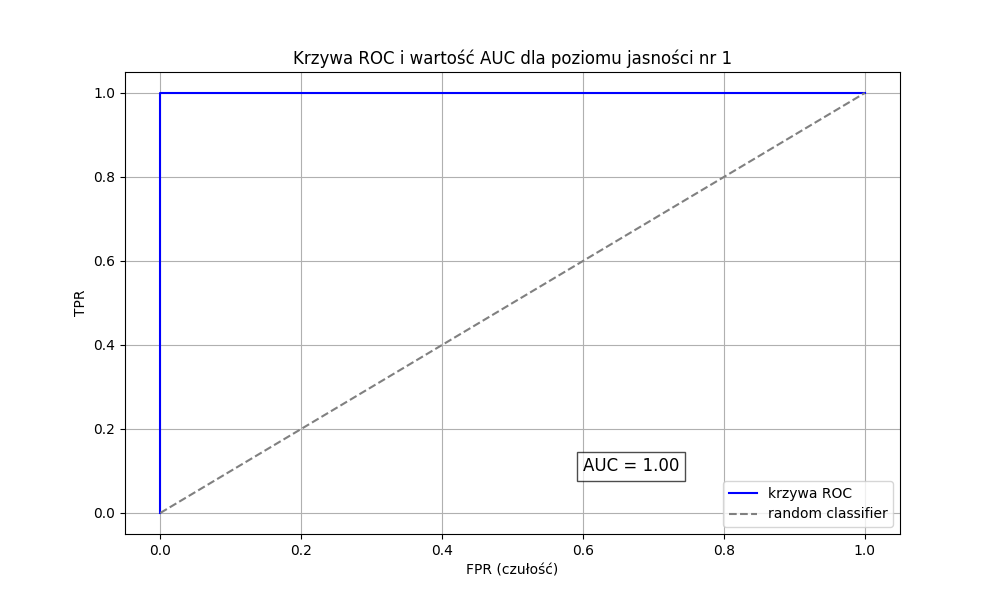
\includegraphics[width=\linewidth]{r_test_dokładności/AUC_charts/1.png}
    \caption{Krzywa ROC i wartość AUC dla poziomu jasności nr 1.}
    \label{fig:ROC-1}
\end{figure}

\begin{figure}[H]
    \centering
    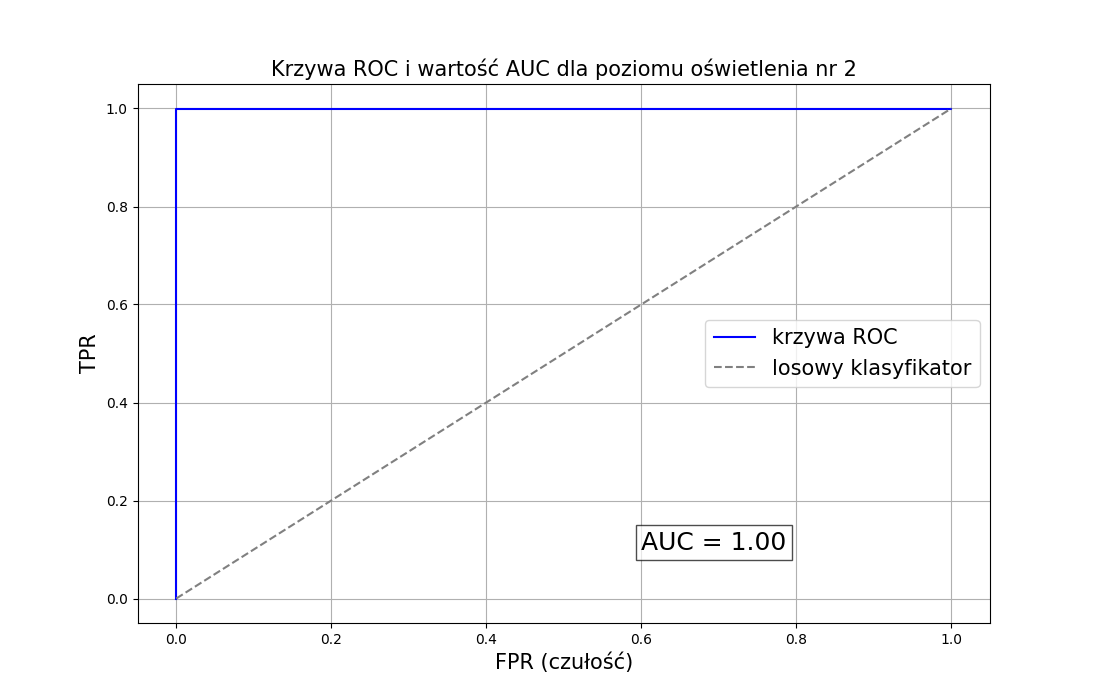
\includegraphics[width=\linewidth]{r_test_dokładności/AUC_charts/2.png}
    \caption{Krzywa ROC i wartość AUC dla poziomu jasności nr 2.}
    \label{fig:ROC-2}
\end{figure}

\begin{figure}[H]
    \centering
    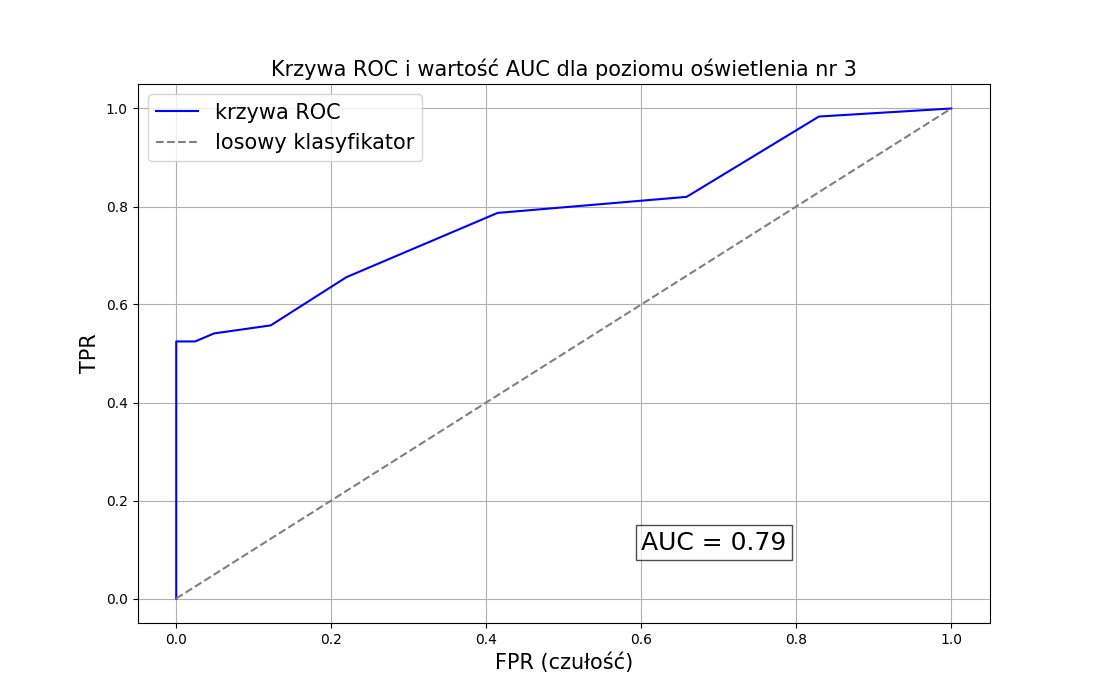
\includegraphics[width=\linewidth]{r_test_dokładności/AUC_charts/3.png}
    \caption{Krzywa ROC i wartość AUC dla poziomu jasności nr 3.}
    \label{fig:ROC-3}
\end{figure}

\begin{figure}[H]
    \centering
    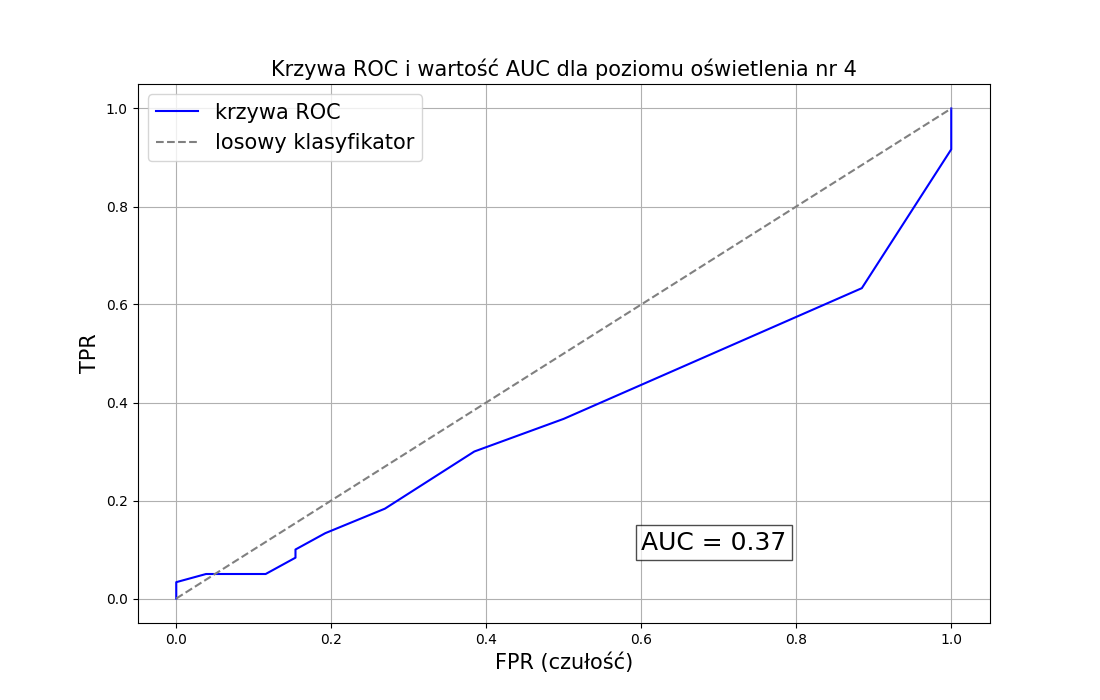
\includegraphics[width=\linewidth]{r_test_dokładności/AUC_charts/4.png}
    \caption{Krzywa ROC i wartość AUC dla poziomu jasności nr 4.}
    \label{fig:ROC-4}
\end{figure}

\begin{figure}[H]
    \centering
    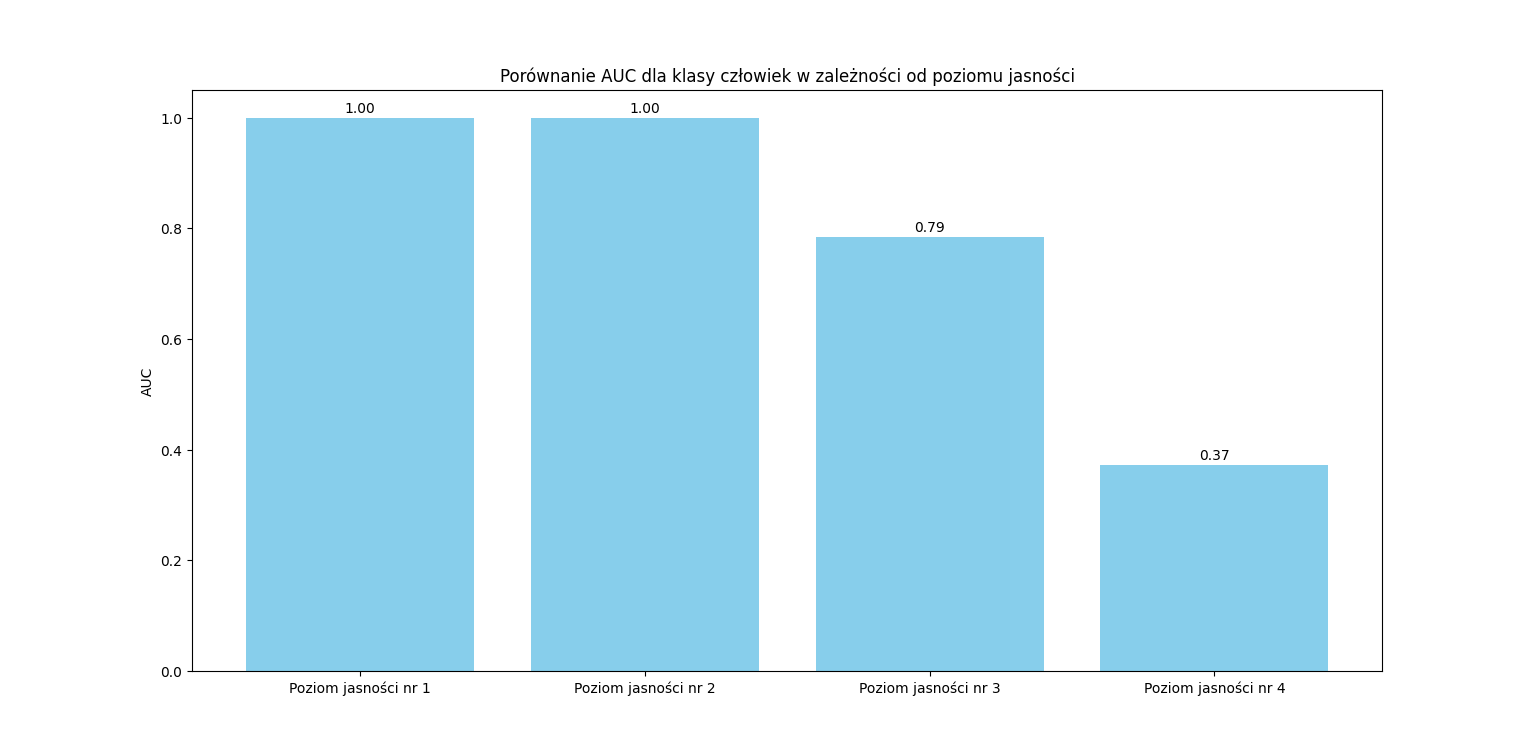
\includegraphics[width=\linewidth]{r_test_dokładności/AUC_charts/porownanieAUC.png}
    \caption{Wykres porównujący wartości AUC dla zbadanych poziomów jasności.}
    \label{fig:AUC}
\end{figure}

Przed wyciągnięciem wniosków z wykresów należy opisać jakościowo wszystkie poziomy oświetlenia. 
\begin{itemize}
    \item \textbf{Poziom nr 1:} Obiekty są bardzo dobrze widoczne. Limonkowe tło pokoju korzystnie wpływa na podkreślenie konturów człowieka. Sprzyja także nasycenie barwy. Oczekuje się i wymaga dobrego wyniku detektora. 
    \item \textbf{Poziom nr 2:} Widoczność równie dobra co dla poziomu nr 1. Różnica nasycenia oraz jasności pomiedzy tymi poziomami jest zdecdowanie mniejsza niż np. róznica miedzy poziomami nr 2 i 3. Oczekuje się i wymaga podobnego wyniku co w przypadku poziomu nr 1.
    \item \textbf{Poziom nr 3:} Poziom ten to wyraźny przeskok w widoczności w porównaniu do poprzednich poziomów. Mimo to ludzkie oko dostrzega człowieka dla każdej klatki kiedy człowiek uznany jest za obecnego. Poziom ten uznaje się za najważniejszy w badaniu.
    \item \textbf{Poziom nr 4:} Obiekty są bardzo słabo widoczne. Dla wielu zdefiniowanych klatek samo ludzkie oko ma problem ze stwierdzeniem obecności człowieka w pomieszczeniu. Z racji tego, przewiduje się złe osiągi modelu. Jest to mało prawdopodobne, iż model dokładniej stwierdzi obiekt niż ludzkie oko. W związku z tym poziom ten nie jest znaczący w analizie i finalnej ocenie modelu dla tego badania. 
\end{itemize}

Jak widać na wykresach na rysunkach \ref{fig:ROC-1} i \ref{fig:ROC-2} model osiągnął wartość idealną --- równą 1. Budzi to zastrzeżenia co do poprawności przygotowanych danych. W rzeczywistośći wartość AUC nie jest równa 1, lecz bardzo bliska 1, więc wartość ta jest efektem zaokrąglenia. Można więc stwierdzić, że w bardzo dobrych warunkach oświetlenia model sprawdza się wzorowo. Jest to przydatna informacja, jeżeli użytkownik sądzi, iż może wykorzystać system w dla celów ważna jest bliska zeru błędnych reakcji systemu. Z uwagi na prosty scenariusz testowy i brak dalszych badań nie rekomenduje się jednak używania systemu w scenariuszach krytycznych takich jak monitoring wizyjny. Natomiast takich zastosowań nie założono w systemie. Teoretyczną wartość dla poziomu nr 3 można uznać za dobrą. W praktyce można interpretować ją różnie. Skalarna wartość jest jednak bardzo ogólną metryką i bardzo wiele zależy od konkretnego ustawienia modelu (np. dostosowania progu ufności -- badania przeprowadzone w następnej części tego rozdziału). Wyniki poziomu nr 4 są, tak jak się tego spodziewano, bardzo złe. Pokazuje to, że w takich warunkach oświetleniowych system ten nie powinien zostać użyty. 

Podsumowując, porównanie to udowodniło spodziewane zachowanie -- coraz gorsze wyniki wraz z pogorszającymi się warunkami oświetlenia, co jest dowodem stabilności modelu. Pokazano również, iż system bardzo dobrze sprawdza się w dobrych warunkach oświetlenia alarm na wejściu do pomiesczenia. Taki system możnaby użyć  np. w sytuacji kiedy obiektyw kamery jest skierowany na wejście sklepu. Powiadamiałby pracowników pracujących na zapleczu, że należy obsłużyć klienta.  
Tak jak to jednak podkreślono, AUC jest bardzo ogólną miarą i w celu dokładniejszwego zbadania modelu, należy posłużyć się innymi metrykami. Samo podejście ze stosowaniem krzywej ROC i wartości AUC wzbudza kontrowersje i wątpliwości, opisane np. w pracach \cite{AUC_critique1}, \cite{AUC_critique2}.






\subsection{Analiza wpływu progu ufności na wyniki detekcji}

